% --- LaTeX Homework Template - S. Venkatraman ---

% --- Set document class and font size ---

\documentclass[letterpaper, 11pt]{article}

% --- Package imports ---

\usepackage{
  amsmath, amsthm, amssymb, mathtools, dsfont,	  % Math typesetting
  graphicx, wrapfig, subfig, float,                  % Figures and graphics formatting
  listings, color, inconsolata, pythonhighlight,     % Code formatting
  fancyhdr, sectsty, hyperref, enumerate, enumitem } % Headers/footers, section fonts, links, lists
  
  \usepackage{tikz}
\usetikzlibrary{positioning}
  
  \tikzset{
  vtx/.style={circle, fill=black, inner sep=1.6pt},
  every picture/.style={>=latex}
}

\usetikzlibrary{positioning,calc}

% --- Page layout settings ---

% Set page margins
\usepackage[left=0.7in, right=0.7in, bottom=1in, top=1.1in, headsep=0.2in]{geometry}

% Anchor footnotes to the bottom of the page
\usepackage[bottom]{footmisc}



% Set line spacing
\renewcommand{\baselinestretch}{1.2}

% Set spacing between paragraphs
\setlength{\parskip}{1.5mm}

% Allow multi-line equations to break onto the next page
\allowdisplaybreaks

% Enumerated lists: make numbers flush left, with parentheses around them
\setlist[enumerate]{wide=0pt, leftmargin=21pt, labelwidth=0pt, align=left}
\setenumerate[1]{label={(\arabic*)}}

% --- Page formatting settings ---

% Set link colors for labeled items (blue) and citations (red)
\hypersetup{colorlinks=true, linkcolor=blue, citecolor=red}

% Make reference section title font smaller
\renewcommand{\refname}{\large\bf{References}}

% --- Settings for printing computer code ---

% Define colors for green text (comments), grey text (line numbers),
% and green frame around code
\definecolor{greenText}{rgb}{0.5, 0.7, 0.5}
\definecolor{greyText}{rgb}{0.5, 0.5, 0.5}
\definecolor{codeFrame}{rgb}{0.5, 0.7, 0.5}

% Define code settings
\lstdefinestyle{code} {
  frame=single, rulecolor=\color{codeFrame},            % Include a green frame around the code
  numbers=left,                                         % Include line numbers
  numbersep=8pt,                                        % Add space between line numbers and frame
  numberstyle=\tiny\color{greyText},                    % Line number font size (tiny) and color (grey)
  commentstyle=\color{greenText},                       % Put comments in green text
  basicstyle=\linespread{1.1}\ttfamily\footnotesize,    % Set code line spacing
  keywordstyle=\ttfamily\footnotesize,                  % No special formatting for keywords
  showstringspaces=false,                               % No marks for spaces
  xleftmargin=1.95em,                                   % Align code frame with main text
  framexleftmargin=1.6em,                               % Extend frame left margin to include line numbers
  breaklines=true,                                      % Wrap long lines of code
  postbreak=\mbox{\textcolor{greenText}{$\hookrightarrow$}\space} % Mark wrapped lines with an arrow
}

% Set all code listings to be styled with the above settings
\lstset{style=code}

% --- Math/Statistics commands ---

% Add a reference number to a single line of a multi-line equation
% Usage: "\numberthis\label{labelNameHere}" in an align or gather environment
\newcommand\numberthis{\addtocounter{equation}{1}\tag{\theequation}}

% Shortcut for bold text in math mode, e.g. $\b{X}$
\let\b\mathbf

% Shortcut for bold Greek letters, e.g. $\bg{\beta}$
\let\bg\boldsymbol

% Shortcut for calligraphic script, e.g. %\mc{M}$
\let\mc\mathcal

% \mathscr{(letter here)} is sometimes used to denote vector spaces
\usepackage[mathscr]{euscript}

% Convergence: right arrow with optional text on top
% E.g. $\converge[w]$ for weak convergence
\newcommand{\converge}[1][]{\xrightarrow{#1}}

% Normal distribution: arguments are the mean and variance
% E.g. $\normal{\mu}{\sigma}$
\newcommand{\normal}[2]{\mathcal{N}\left(#1,#2\right)}

% Uniform distribution: arguments are the left and right endpoints
% E.g. $\unif{0}{1}$
\newcommand{\unif}[2]{\text{Uniform}(#1,#2)}

% Independent and identically distributed random variables
% E.g. $ X_1,...,X_n \iid \normal{0}{1}$
\newcommand{\iid}{\stackrel{\smash{\text{iid}}}{\sim}}

% Equality: equals sign with optional text on top
% E.g. $X \equals[d] Y$ for equality in distribution
\newcommand{\equals}[1][]{\stackrel{\smash{#1}}{=}}

% Math mode symbols for common sets and spaces. Example usage: $\R$
\newcommand{\R}{\mathbb{R}}   % Real numbers
\newcommand{\C}{\mathbb{C}}   % Complex numbers
\newcommand{\Q}{\mathbb{Q}}   % Rational numbers
\newcommand{\Z}{\mathbb{Z}}   % Integers
\newcommand{\N}{\mathbb{N}}   % Natural numbers
\newcommand{\F}{\mathcal{F}}  % Calligraphic F for a sigma algebra
\newcommand{\El}{\mathcal{L}} % Calligraphic L, e.g. for L^p spaces

% Math mode symbols for probability
\newcommand{\pr}{\mathbb{P}}    % Probability measure
\newcommand{\E}{\mathbb{E}}     % Expectation, e.g. $\E(X)$
\newcommand{\var}{\text{Var}}   % Variance, e.g. $\var(X)$
\newcommand{\cov}{\text{Cov}}   % Covariance, e.g. $\cov(X,Y)$
\newcommand{\corr}{\text{Corr}} % Correlation, e.g. $\corr(X,Y)$
\newcommand{\B}{\mathcal{B}}    % Borel sigma-algebra

% Other miscellaneous symbols
\newcommand{\tth}{\text{th}}	% Non-italicized 'th', e.g. $n^\tth$
\newcommand{\Oh}{\mathcal{O}}	% Big-O notation, e.g. $\O(n)$
\newcommand{\1}{\mathds{1}}	% Indicator function, e.g. $\1_A$

% Additional commands for math mode
\DeclareMathOperator*{\argmax}{argmax}    % Argmax, e.g. $\argmax_{x\in[0,1]} f(x)$
\DeclareMathOperator*{\argmin}{argmin}    % Argmin, e.g. $\argmin_{x\in[0,1]} f(x)$
\DeclareMathOperator*{\spann}{Span}       % Span, e.g. $\spann\{X_1,...,X_n\}$
\DeclareMathOperator*{\bias}{Bias}        % Bias, e.g. $\bias(\hat\theta)$
\DeclareMathOperator*{\ran}{ran}          % Range of an operator, e.g. $\ran(T) 
\DeclareMathOperator*{\dv}{d\!}           % Non-italicized 'with respect to', e.g. $\int f(x) \dv x$
\DeclareMathOperator*{\diag}{diag}        % Diagonal of a matrix, e.g. $\diag(M)$
\DeclareMathOperator*{\trace}{trace}      % Trace of a matrix, e.g. $\trace(M)$

% Numbered theorem, lemma, etc. settings - e.g., a definition, lemma, and theorem appearing in that 
% order in Section 2 will be numbered Definition 2.1, Lemma 2.2, Theorem 2.3. 
% Example usage: \begin{theorem}[Name of theorem] Theorem statement \end{theorem}
\theoremstyle{definition}
\newtheorem{theorem}{Theorem}[section]
\newtheorem{proposition}[theorem]{Proposition}
\newtheorem{lemma}[theorem]{Lemma}
\newtheorem{corollary}[theorem]{Corollary}
\newtheorem{definition}[theorem]{Definition}
\newtheorem{example}[theorem]{Example}
\newtheorem{remark}[theorem]{Remark}

% Un-numbered theorem, lemma, etc. settings
% Example usage: \begin{lemma*}[Name of lemma] Lemma statement \end{lemma*}
\newtheorem*{theorem*}{Theorem}
\newtheorem*{proposition*}{Proposition}
\newtheorem*{lemma*}{Lemma}
\newtheorem*{corollary*}{Corollary}
\newtheorem*{definition*}{Definition}
\newtheorem*{example*}{Example}
\newtheorem*{remark*}{Remark}
\newtheorem*{claim}{Claim}
\newcommand{\Tau}{\mathcal{T}}
\newcommand{\PSet}{\mathcal{P}}





% --- Left/right header text (to appear on every page) ---

% Include a line underneath the header, no footer line
\pagestyle{fancy}
\renewcommand{\footrulewidth}{0pt}
\renewcommand{\headrulewidth}{0.4pt}

% Left header text: course name/assignment number
\lhead{MAM4000W, Graph Theory -- Comprehension Test 1}

% Right header text: your name
\rhead{Alex Cristaudo, CRSALE010}

% --- Document starts here ---

\begin{document}
~\\
To understand the notation we will use, look at the following example, $K_3 \times K_4$



\begin{center}

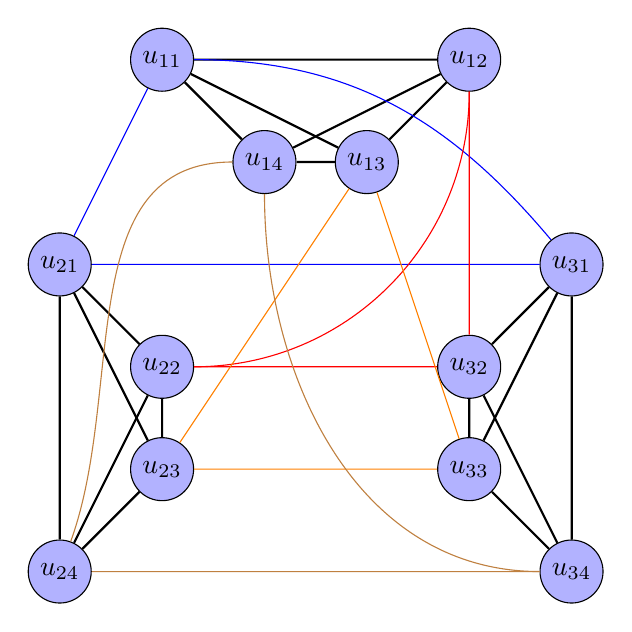
\begin{tikzpicture}[scale=1.3]

  % --- node style ---
  \tikzset{vtx/.style={circle, fill=blue!30, draw, minimum size=8mm, inner sep=0pt}}
  \tikzset{edge/.style={thick}}
  
  \node[vtx] (u11) at (1,4) {$u_{11}$};
    \node[vtx] (u12) at (4,4) {$u_{12}$};
      \node[vtx] (u13) at (3,3) {$u_{13}$};
        \node[vtx] (u14) at (2,3) {$u_{14}$};
        
        
  \node[vtx] (u21) at (0,2) {$u_{21}$};
    \node[vtx] (u22) at (1,1) {$u_{22}$};
      \node[vtx] (u23) at (1,0) {$u_{23}$};
        \node[vtx] (u24) at (0,-1) {$u_{24}$};
        
        
  \node[vtx] (u31) at (5,2) {$u_{31}$};
    \node[vtx] (u32) at (4,1) {$u_{32}$};
      \node[vtx] (u33) at (4,0) {$u_{33}$};
        \node[vtx] (u34) at (5,-1) {$u_{34}$};
        
    \draw[edge] (u11) -- (u14) -- (u13) -- (u12) -- (u11);
        \draw[edge] (u11) -- (u13);
                \draw[edge] (u12) -- (u14);
                
                
    \draw[edge] (u21) -- (u24) -- (u23) -- (u22) -- (u21);
        \draw[edge] (u21) -- (u23);
                \draw[edge] (u22) -- (u24);


    \draw[edge] (u31) -- (u34) -- (u33) -- (u32) -- (u31);
        \draw[edge] (u31) -- (u33);
                \draw[edge] (u32) -- (u34);

\draw[thin, blue] (u11) -- (u21) -- (u31);
\draw[thin, blue] (u31) to[in = 0, out = 130] (u11);

\draw[thin, red] (u12) to[in =0, out = -90] (u22);
\draw[thin, red] (u22) -- (u32) -- (u12);

\draw[thin, orange] (u13) -- (u23) -- (u33) -- (u13);

\draw[thin, brown] (u24) -- (u34);
\draw[thin, brown] (u14) to[in = 70, out = 180] (u24);
\draw[thin, brown] (u14) to[in = 180, out = -90] (u34);


\end{tikzpicture}

\end{center}
We will denote the vertices $V(K_m \times K_n) := \{ u_{ij} : 1\le i \le m, 1 \le j \le n\}$ where we have edges:
\[
u_{ij}u_{ik}, \quad 1 \le i \le m, 1 \le j, k \le n, j \ne k \quad \quad \quad (1)
\]
\[
u_{ij}u_{kj}, \quad 1 \le i,k \le m, 1 \le j \le n, i \ne k \quad \quad \quad (2)
\]
That is, vertices in the same $K_n$ part of the graph share the same first index, and the vertices in the same $K_mx$ part of the graph share the same second index. ~\\~\\Note that $F_1 \cong mK_n$ is the subgraph of $G$ obtained by removing edges described in $(2)$, the $K_n$ subgraphs of $G$ that are disconnected. Graphically, using the example above, $F_1$ is the face:


\begin{center}

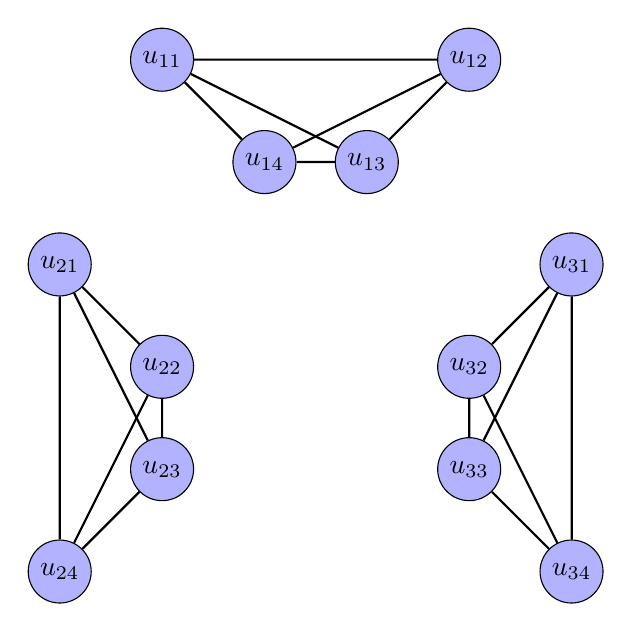
\begin{tikzpicture}[scale=1.3]

  % --- node style ---
  \tikzset{vtx/.style={circle, fill=blue!30, draw, minimum size=8mm, inner sep=0pt}}
  \tikzset{edge/.style={thick}}
  
  \node[vtx] (u11) at (1,4) {$u_{11}$};
    \node[vtx] (u12) at (4,4) {$u_{12}$};
      \node[vtx] (u13) at (3,3) {$u_{13}$};
        \node[vtx] (u14) at (2,3) {$u_{14}$};
        
        
  \node[vtx] (u21) at (0,2) {$u_{21}$};
    \node[vtx] (u22) at (1,1) {$u_{22}$};
      \node[vtx] (u23) at (1,0) {$u_{23}$};
        \node[vtx] (u24) at (0,-1) {$u_{24}$};
        
        
  \node[vtx] (u31) at (5,2) {$u_{31}$};
    \node[vtx] (u32) at (4,1) {$u_{32}$};
      \node[vtx] (u33) at (4,0) {$u_{33}$};
        \node[vtx] (u34) at (5,-1) {$u_{34}$};
        
    \draw[edge] (u11) -- (u14) -- (u13) -- (u12) -- (u11);
        \draw[edge] (u11) -- (u13);
                \draw[edge] (u12) -- (u14);
                
                
    \draw[edge] (u21) -- (u24) -- (u23) -- (u22) -- (u21);
        \draw[edge] (u21) -- (u23);
                \draw[edge] (u22) -- (u24);


    \draw[edge] (u31) -- (u34) -- (u33) -- (u32) -- (u31);
        \draw[edge] (u31) -- (u33);
                \draw[edge] (u32) -- (u34);


\end{tikzpicture}

\end{center}
A set $S \subseteq V(G)$ is dominating $F_1$ iff $N[S] = V(F_1)$ in $F_1$. $F_1$ consists of $m$ disconnected components isomorphic to $K_n$.  So write $F_1 = \bigcup \limits _{i=1}^m C_i$ where each $C_i \cong K_n$ is the component with vertices $\{u_{ij}: 1\le j \le n\}$. In order for $S$ to dominate $F_1$, $S$ must then contain at least one vertex from each component.  Containing a vertex $v \in C_i$ for some $1 \le i \le m$ means that every vertex in $C_i$ is in $N[S]$ (since $C_i$ is complete). Note that two vertices are in different components in $F_1$ if their first index differs. Choosing a vertex from every $C_i$, $1 \le i \le m$, means choosing a set vertices such that every $1,2,...,m$ is a first index of some vertex.\\ ~\\ We have that $F_2 \cong nK_m$ is the subgraph of $G$ obtained by removing edges described in $(1)$, with $F_2 = \bigcup \limits _{j=1}^nD_j$ where each $D_j \cong K_m$ is the component with vertices $\{u_{ij}: 1 \le i \le m\}$. Again, using the example above, $F_2$ is the face:
\begin{center}

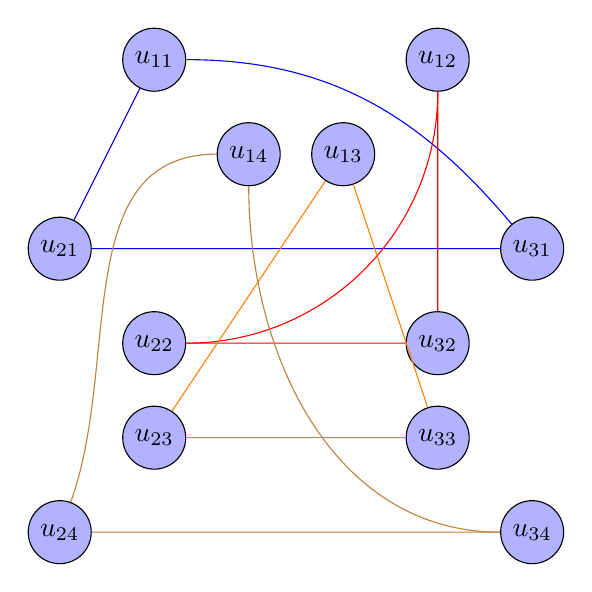
\begin{tikzpicture}[scale=1.2]

  % --- node style ---
  \tikzset{vtx/.style={circle, fill=blue!30, draw, minimum size=8mm, inner sep=0pt}}
  \tikzset{edge/.style={thick}}
  
  \node[vtx] (u11) at (1,4) {$u_{11}$};
    \node[vtx] (u12) at (4,4) {$u_{12}$};
      \node[vtx] (u13) at (3,3) {$u_{13}$};
        \node[vtx] (u14) at (2,3) {$u_{14}$};
        
        
  \node[vtx] (u21) at (0,2) {$u_{21}$};
    \node[vtx] (u22) at (1,1) {$u_{22}$};
      \node[vtx] (u23) at (1,0) {$u_{23}$};
        \node[vtx] (u24) at (0,-1) {$u_{24}$};
        
        
  \node[vtx] (u31) at (5,2) {$u_{31}$};
    \node[vtx] (u32) at (4,1) {$u_{32}$};
      \node[vtx] (u33) at (4,0) {$u_{33}$};
        \node[vtx] (u34) at (5,-1) {$u_{34}$};
        
\draw[thin, blue] (u11) -- (u21) -- (u31);
\draw[thin, blue] (u31) to[in = 0, out = 130] (u11);

\draw[thin, red] (u12) to[in =0, out = -90] (u22);
\draw[thin, red] (u22) -- (u32) -- (u12);

\draw[thin, orange] (u13) -- (u23) -- (u33) -- (u13);

\draw[thin, brown] (u24) -- (u34);
\draw[thin, brown] (u14) to[in = 70, out = 180] (u24);
\draw[thin, brown] (u14) to[in = 180, out = -90] (u34);


\end{tikzpicture}

\end{center}
As explained above, in order for a vertex-set $S$ to dominate $F_2$, $S$ must contain at least one vertex from each component $D_j$, and containing a vertex $v \in D_j$, for some $1 \le j \le n$, means that every vertex in $D_j$ is in $N[S]$. Note that two vertices are in different components in $F_2$ if their second index differs. Choosing a vertex from every $D_j$, $1 \le j \le n$, means choosing a set vertices such that every $1,2,...,n$ is a second index of some vertex.~\\ ~\\
So for a set $S$ to be a global dominating set of $G$ with respect to $\{F_1, F_2\}$, $S$ must contain at least one vertex from every $C_i$ and $D_j$, for $1 \le i \le m, 1 \le j \le n$. Consider $S$ in the following 2 cases and we will show it is a minimum global dominating set.  \[
1. \ \ m < n \quad \quad \quad S = \{u_{11}, u_{22}, u_{33}, ..., u_{mm}, u_{1,m+1}, ..., u_{1n}\}
\]
\[
2. \ \ m = n \quad \quad \quad \quad \quad \quad \ \quad \quad \quad S = \{u_{11}, u_{22}, u_{33}, ..., u_{mm}\}
\]
In both these cases, this set contains exactly $n$ vertices, one from each $D_j$, $1 \le j \le n$, so it is a minimum. It dominates $F_1$ and $F_2$ since it contains a vertex from every component $C_i$ and $D_j$, $1 \le i \le m, 1 \le j \le n$. ~\\
If $m > n$, we use 
\[
S = \{u_{11}, u_{22}, u_{33}, ..., u_{nn}, u_{n+1, 1}, ..., u_{m1}\}
\]
This set contains exactly $m$ vertices, one from each $C_i$, $1 \le i \le m$, so it is a minimum. It dominates $F_1$ and $F_2$ since it contains a vertex from every component $C_i$ and $D_j$, $1 \le i \le m, 1 \le j \le n$. ~\\
~\\So $\gamma (K_m \times K_n, \{F_1, F_2\}) = \max \{n,m\}$
\end{document}
